\documentclass{article}

\usepackage{graphicx}
\usepackage{tikz}
\usepackage{tikzsymbols}
\usetikzlibrary{calc,patterns,shapes.geometric}
\pagestyle{empty}
\usepackage[margin=0pt]{geometry}
\geometry{papersize={14in,12in}}

\def\centerarc[#1](#2)(#3:#4:#5){\draw[#1] ($(#2)+({#5*cos(#3)},{#5*sin(#3)})$) arc (#3:#4:#5);}

\begin{document}
	\begin{figure}
		\centering
		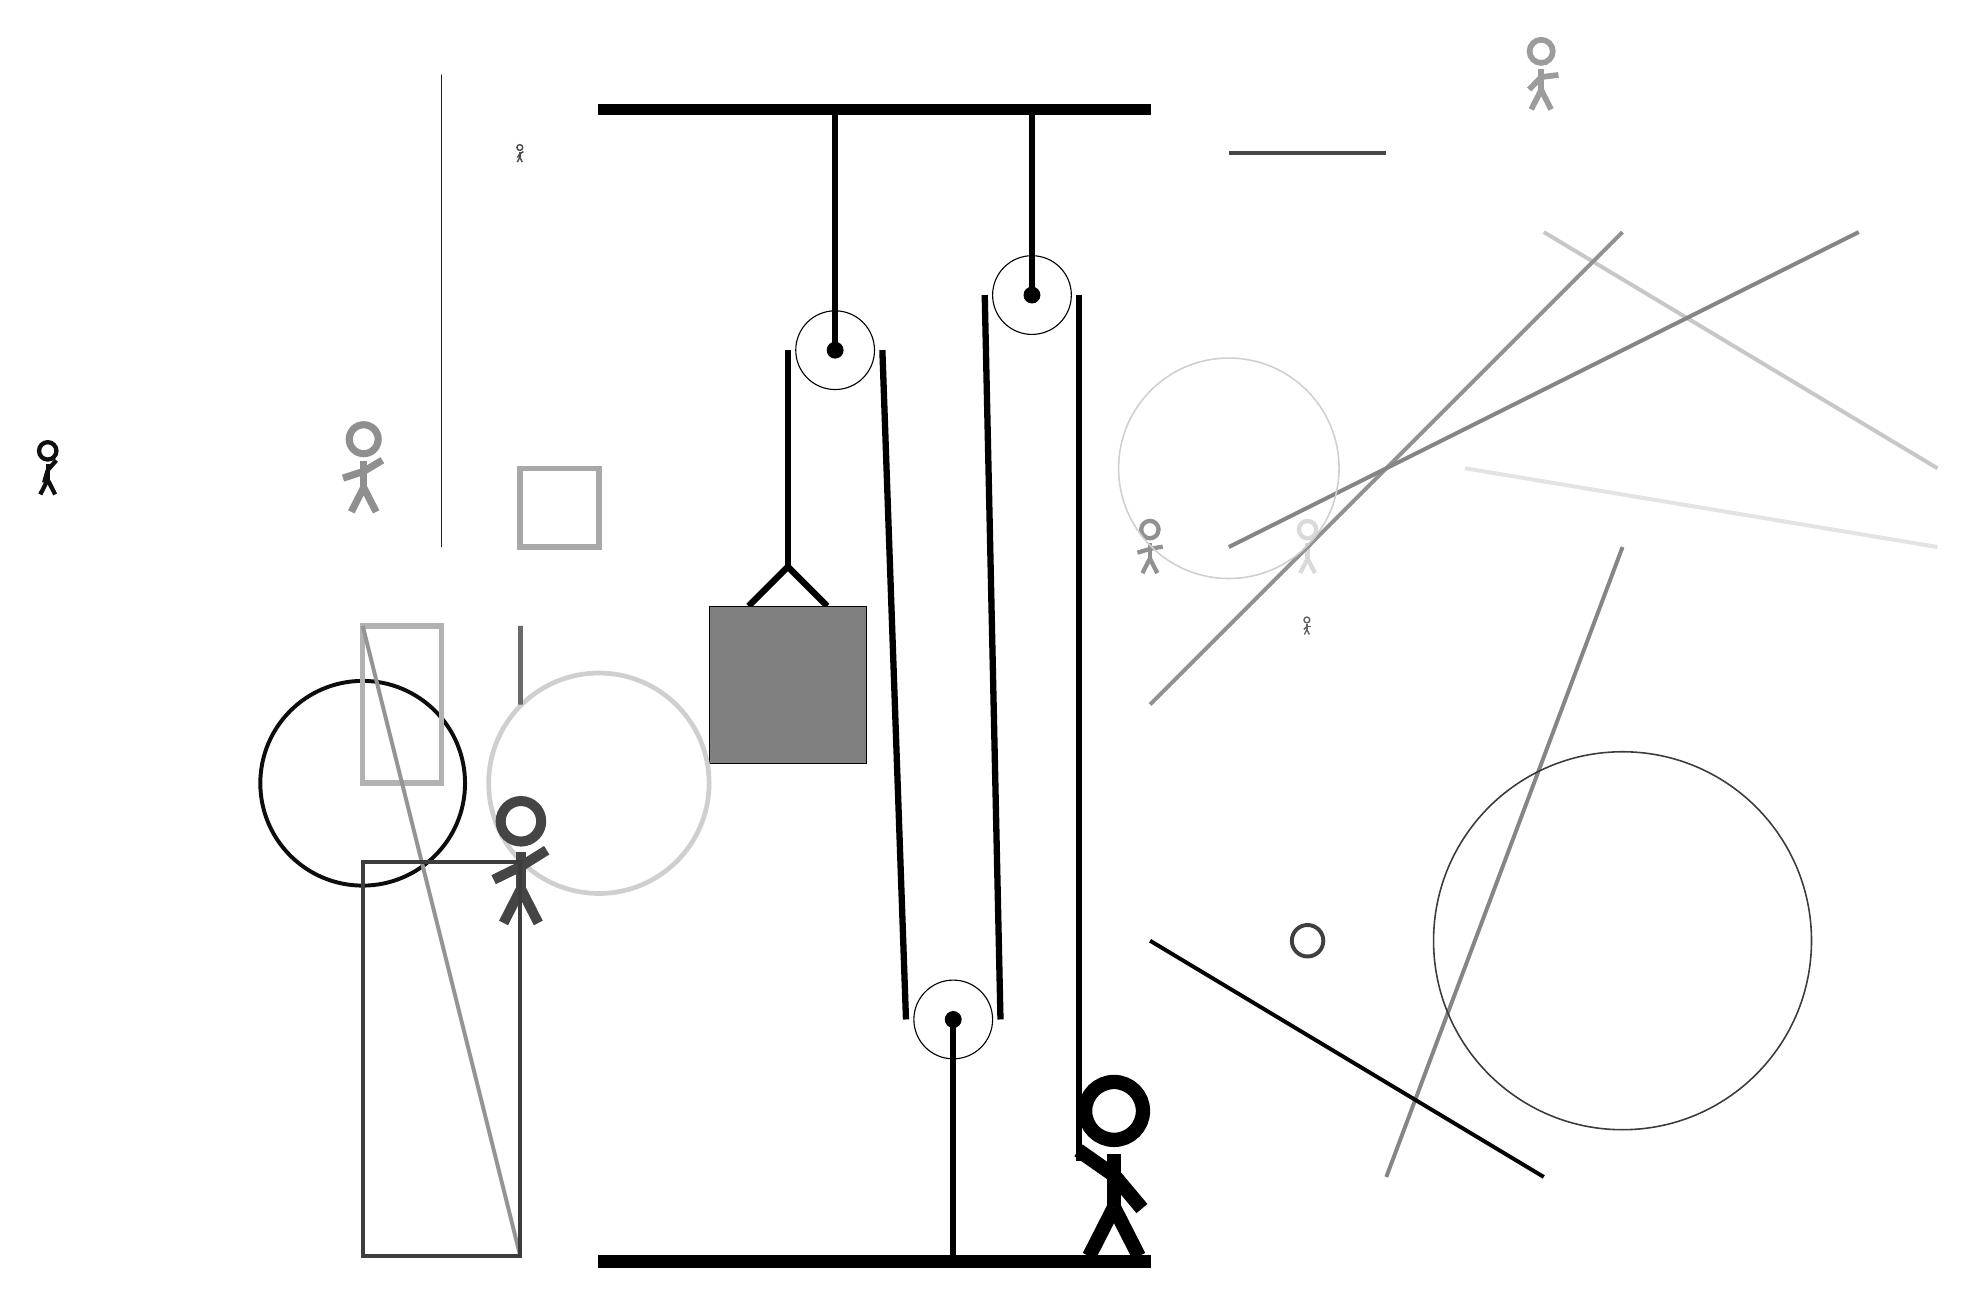
\begin{tikzpicture}
			%%%%% START %%%%%
			
			\draw[fill=black] (-2, 11.5) rectangle (5, 11.625);
			
			\draw (1, 8.5) circle (0.5);
			\draw[fill=black] (1, 8.5) circle (0.1);
			\draw[line width=0.8mm]  (1, 11.5) -- (1, 8.5);
			
			\draw[fill=white](2.5, 0.0) circle (0.5);
			\draw[fill=black] (2.5, 0.0) circle (0.1);
			\draw[line width=0.8mm]  (2.5, -3) -- (2.5, 0.0);
			
			\draw[fill=white](3.5, 9.2) circle (0.5);
			\draw[fill=black] (3.5, 9.2) circle (0.1);
			\draw[line width=0.8mm] (3.5, 11.5) -- (3.5, 9.2);
			
			\draw[line width=0.8mm] (-0.1, 5.25) -- (0.4, 5.75) -- (0.9, 5.25);
			\draw[fill=black!50] (-0.6, 5.25) rectangle (1.4, 3.25);
			
			\draw[line width=0.8mm] (0.4, 8.5) -- (0.4, 5.75);
			\centerarc[line width=0.8mm](1, 8.5)(0:180:0.6);
			\draw[line width=0.8mm](1.6, 8.5) -- (1.9, 0.0);
			\centerarc[line width=0.8mm](2.5, 0.0)(180:360:0.6);
			\draw[line width=0.8mm](3.1, 0.0) -- (2.9, 9.2);
			\centerarc[line width=0.8mm](3.5, 9.2)(0:180:0.6);
			\draw[line width=0.8mm](4.1, 9.2) -- (4.1, -1.8);
			
			\node at (4.5, -1.9) {\Strichmaxerl[10][-35][-50]};
			
			\draw[line width=0.5mm, color=black!48](8, -2) -- (11, 6);
			
			\draw[line width=0.5mm, color=black!98](10, -2) -- (5, 1);
			\draw [line width=0.5mm, color=black!95](-5, 3) circle (1.3);
			\draw[line width=0.5mm, color=black!22](10, 10) -- (15, 7);
			\node[line width=0.6mm, color=black!61] at (7, 5) {\Strichmaxerl[1][46][0]};
			\node[line width=0.4mm, color=black!15] at (7, 6) {\Strichmaxerl[3][89][59]};
			\draw [line width=0.2mm, color=black!77](11, 1) circle (2.4);
			\draw[line width=0.7mm, color=black!34] (-3, 6) rectangle (-2, 7);
			\draw [line width=0.6mm, color=black!19](-2, 3) circle (1.4);
			
			\node[line width=0.2mm, color=black!44] at (-5, 7) {\Strichmaxerl[5][18][31]};
			\draw [line width=0.5mm, color=black!75](7, 1) circle (0.2);
			\node[line width=0.6mm, color=black!43] at (5, 6) {\Strichmaxerl[3][17][10]};
			\node[line width=0.4mm, color=black!39] at (10, 12) {\Strichmaxerl[4][46][7]};
			\draw[line width=0.5mm, color=black!43](5, 4) -- (11, 10);
			\draw[line width=0.5mm, color=black!48](6, 6) -- (14, 10);
			\draw[line width=0.7mm, color=black!30] (-4, 3) rectangle (-5, 5);
			
			\draw[line width=0.5mm, color=black!72](8, 11) -- (6, 11);
			\draw[line width=0.6mm, color=black!59] (-3, 5) rectangle (-3, 4);
			\node[line width=0.7mm, color=black!70] at (-3, 11) {\Strichmaxerl[1][55][34]};
			\draw[line width=0.5mm, color=black!11](9, 7) -- (15, 6);
			\node[line width=0.3mm, color=black!73] at (-3, 2) {\Strichmaxerl[7][26][32]};
			\draw [line width=0.2mm, color=black!19](6, 7) circle (1.4);
			\draw[line width=0.5mm, color=black!42](-3, -3) -- (-5, 5);
			\draw[line width=0.3mm, color=black!27] (-4, 4) rectangle (-4, 4);
			\draw[line width=0.5mm, color=black!76] (-3, 2) rectangle (-5, -3);
			
			\draw[line width=0.2mm, color=black!89] (-4, 12) rectangle (-4, 6);
			
			\node[line width=0.5mm, color=black!94] at (-9, 7) {\Strichmaxerl[3][74][49]};
			
			\draw[fill=black] (-2, -3) rectangle (5, -3.15);
			
			%%%%% END %%%%%
		\end{tikzpicture}
	\end{figure}	
\end{document}